%
% ---------------------------------------------------------------
% Copyright (C) 2012-2018 Gang Li
% ---------------------------------------------------------------
%
% This work is the default powerdot-tuliplab style test file and may be
% distributed and/or modified under the conditions of the LaTeX Project Public
% License, either version 1.3 of this license or (at your option) any later
% version. The latest version of this license is in
% http://www.latex-project.org/lppl.txt and version 1.3 or later is part of all
% distributions of LaTeX version 2003/12/01 or later.
%
% This work has the LPPL maintenance status "maintained".
%
% This Current Maintainer of this work is Gang Li.
%
%

\documentclass[
 size=14pt,
 paper=smartboard,  %a4paper, smartboard, screen
 mode=present, 		%present, handout, print
 display=slides, 	% slidesnotes, notes, slides
 style=tuliplab,  	% TULIP Lab style
 pauseslide,
 fleqn,leqno]{powerdot}


\usepackage{cancel}
\usepackage{caption}
\usepackage{stackengine}
\usepackage{smartdiagram}
\usepackage{attrib}
\usepackage{amssymb}
\usepackage{amsmath} 
\usepackage{amsthm} 
\usepackage{mathtools}
\usepackage{rotating}
\usepackage{graphicx}
\usepackage{boxedminipage}
\usepackage{rotate}
\usepackage{calc}
\usepackage[absolute]{textpos}
\usepackage{psfrag,overpic}
\usepackage{fouriernc}
\usepackage{pstricks,pst-3d,pst-grad,pstricks-add,pst-text,pst-node,pst-tree}
\usepackage{moreverb,epsfig,subfigure}
\usepackage{color}
\usepackage{booktabs}
\usepackage{etex}
\usepackage{breqn}
\usepackage{multirow}
\usepackage{natbib}
\usepackage{bibentry}
\usepackage{gitinfo2}
\usepackage{siunitx}
\usepackage{nicefrac}
%\usepackage{geometry}
%\geometry{verbose,letterpaper}
\usepackage{media9}
\usepackage{animate}
%\usepackage{movie15}
\usepackage{auto-pst-pdf}

\usepackage{breakurl}
\usepackage{fontawesome}
\usepackage{xcolor}
\usepackage{multicol}



\usepackage{verbatim}
\usepackage[utf8]{inputenc}
\usepackage{dtk-logos}
\usepackage{tikz}
\usepackage{adigraph}
%\usepackage{tkz-graph}
\usepackage{hyperref}
%\usepackage{ulem}
\usepackage{pgfplots}
\usepackage{verbatim}
\usepackage{fontawesome}


\usepackage{todonotes}
% \usepackage{pst-rel-points}
\usepackage{animate}
\usepackage{fontawesome}

\usepackage{listings}
\lstset{frameround=fttt,
frame=trBL,
stringstyle=\ttfamily,
backgroundcolor=\color{yellow!20},
basicstyle=\footnotesize\ttfamily}
\lstnewenvironment{code}{
\lstset{frame=single,escapeinside=`',
backgroundcolor=\color{yellow!20},
basicstyle=\footnotesize\ttfamily}
}{}


\usepackage{hyperref}
\hypersetup{ % TODO: PDF meta Data
  pdftitle={Presentation Title},
  pdfauthor={Gang Li},
  pdfpagemode={FullScreen},
  pdfborder={0 0 0}
}


% \usepackage{auto-pst-pdf}
% package to show source code

\definecolor{LightGray}{rgb}{0.9,0.9,0.9}
\newlength{\pixel}\setlength\pixel{0.000714285714\slidewidth}
\setlength{\TPHorizModule}{\slidewidth}
\setlength{\TPVertModule}{\slideheight}
\newcommand\highlight[1]{\fbox{#1}}
\newcommand\icite[1]{{\footnotesize [#1]}}

\newcommand\twotonebox[2]{\fcolorbox{pdcolor2}{pdcolor2}
{#1\vphantom{#2}}\fcolorbox{pdcolor2}{white}{#2\vphantom{#1}}}
\newcommand\twotoneboxo[2]{\fcolorbox{pdcolor2}{pdcolor2}
{#1}\fcolorbox{pdcolor2}{white}{#2}}
\newcommand\vpspace[1]{\vphantom{\vspace{#1}}}
\newcommand\hpspace[1]{\hphantom{\hspace{#1}}}
\newcommand\COMMENT[1]{}

\newcommand\placepos[3]{\hbox to\z@{\kern#1
        \raisebox{-#2}[\z@][\z@]{#3}\hss}\ignorespaces}

\renewcommand{\baselinestretch}{1.2}


\newcommand{\draftnote}[3]{
	\todo[author=#2,color=#1!30,size=\footnotesize]{\textsf{#3}}	}
% TODO: add yourself here:
%
\newcommand{\gangli}[1]{\draftnote{blue}{GLi:}{#1}}
\newcommand{\shaoni}[1]{\draftnote{green}{sn:}{#1}}
\newcommand{\gliMarker}
	{\todo[author=GLi,size=\tiny,inline,color=blue!40]
	{Gang Li has worked up to here.}}
\newcommand{\snMarker}
	{\todo[author=Sn,size=\tiny,inline,color=green!40]
	{Shaoni has worked up to here.}}

%%%%%%%%%%%%%%%%%%%%%%%%%%%%%%%%%%%%%%%%%%%%%%%%%%%%%%%%%%%%%%%%%%%%%%%%
% title
% TODO: Customize to your Own Title, Name, Address
%
\title{San Francisco Crime classification}
\author{
Jia Huang
\\
\\Xi'an Shiyou University
%\\Deakin University
\\Chinese Academy of Sciences
%\\ \today
}
%\date{\gitCommitterDate}


% Customize the setting of slides
\pdsetup{
% TODO: Customize the left footer, and right footer
rf=\href{http://www.tulip.org.au}{
Last Changed by: \textsc{\gitCommitterName}\ \gitVtagn-\gitAbbrevHash\ (\gitAuthorDate)
},
cf={San Francisco Crime classification},
}


\begin{document}

\maketitle

%\begin{slide}{Overview}
%\tableofcontents[content=sections]
%\end{slide}


%%==========================================================================================
%%
\begin{slide}[toc=,bm=]{Overview}
\tableofcontents[content=currentsection,type=1]
\end{slide}
%%
%%==========================================================================================


\section{Project Overview}


%%==========================================================================================
%%
\begin{slide}{Project Background And Purpose}
\begin{center}
\twotonebox{\rotatebox{95}{Defn}}{\parbox{.89\textwidth}
{
\begin{itemize}
\item Background
\\From 1934 to 1963, San Francisco was infamous for housing
some of the world's most notorious criminals on the 
inescapable island of Alcatraz. Today, the city is known
more for its tech scene than its criminal past. But, with 
rising wealth inequality, housing shortages, and a proliferation
of expensive digital toys riding BART to work, there is no 
scarcity of crime in the city by the bay. From Sunset to SOMA, 
and Marina to Excelsior, this dataset provides nearly 12 years
of crime reports from across all of San Francisco's neighborhoods.
~\\
\item Purpose
\\predict the category of crime that occurred, given the time 
and location visualize the city and crimes (see Mapping and 
Visualizing Violent Crime for inspiration) Content.
\end{itemize}
}}

\end{center}
\bigskip
\begin{center}
\begin{tabular}{c| c c c c }
\toprule
\midrule

\bottomrule
\end{tabular}
\end{center}
\bigskip

%%==========================================================================================
\begin{note}
First, I will introduce the problem definition.
In the real life,
a teacher may be interested in the characteristics that
make one student obvious different from others.
Or,
NBA sports coaches would prefer to
know the advantages and disadvantages of one player.
Here, the player can be regarded as a query object.

For example, team A has five players,
each player has four features.
The NBA sports coaches may want to know the features of
player $1$ that are different from others.

The above example can be seen as outlying aspects mining.
The main purpose of outlying aspects mining is to identify
the outstanding features of the query object.
\end{note}
%%==========================================================================================

\end{slide}
%%
%%==========================================================================================


%%
%%==========================================================================================


\section{Data Pre-Processing}


%%==========================================================================================
%%
\begin{slide}{Date Processing}
%Related Work - Outlying Aspects Mining
This dataset contains incidents derived from 
SFPD Crime Incident Reporting system. The data 
ranges from 1/1/2003 to 5/13/2015. The training 
set and test set rotate every week, meaning 
week 1,3,5,7... belong to test set, week 2,4,6,8 
belong to training set. There are 9 variables.


\bigskip





%%==========================================================================================
\begin{note}
Let me introduce two existing methods:
Feature selection and score-and-search.

For feature selection,
the query point can be regarded as positive class and
the rest of the data can be regarded as negative class,
selected the features that best distinguish the two classes.

The advantages of this method are easy to operate,
and it's able to resolve dimensionality bias.
However, it has some drawbacks.
Firstly,
positive and negative classes are Not balanced,
secondly,
it can't quantify the outlying degree correctly.
Most importantly,
it doesn't identify group outlying aspects.
\end{note}
%%==========================================================================================

\end{slide}
%%
%%==========================================================================================

%%
%%==========================================================================================
\begin{slide}{Feature Item}
By making a comprehensive analysis of the nine
characteristic items in the data set mentioned 
above,we can reach the following conclusions:


\bigskip

\begin{figure}[htbp]
  \centering
  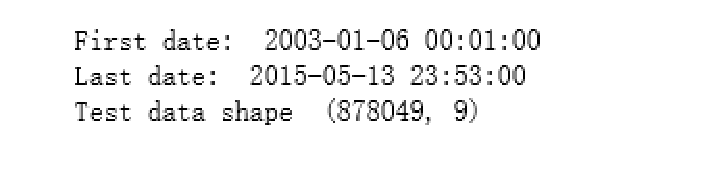
\includegraphics[width=1\textwidth]{kaggle/1.eps}
  \caption{}
\end{figure}
\setlength{\parindent}{2em}The data range was from 1/1/2003 to 5/13/2015, and 
a data training set containing nine feature items and 87,8049 
samples was created.
\end{slide}

%%
%%==========================================================================================
\begin{slide}{Features Item}
  \begin{figure}
    \centering
    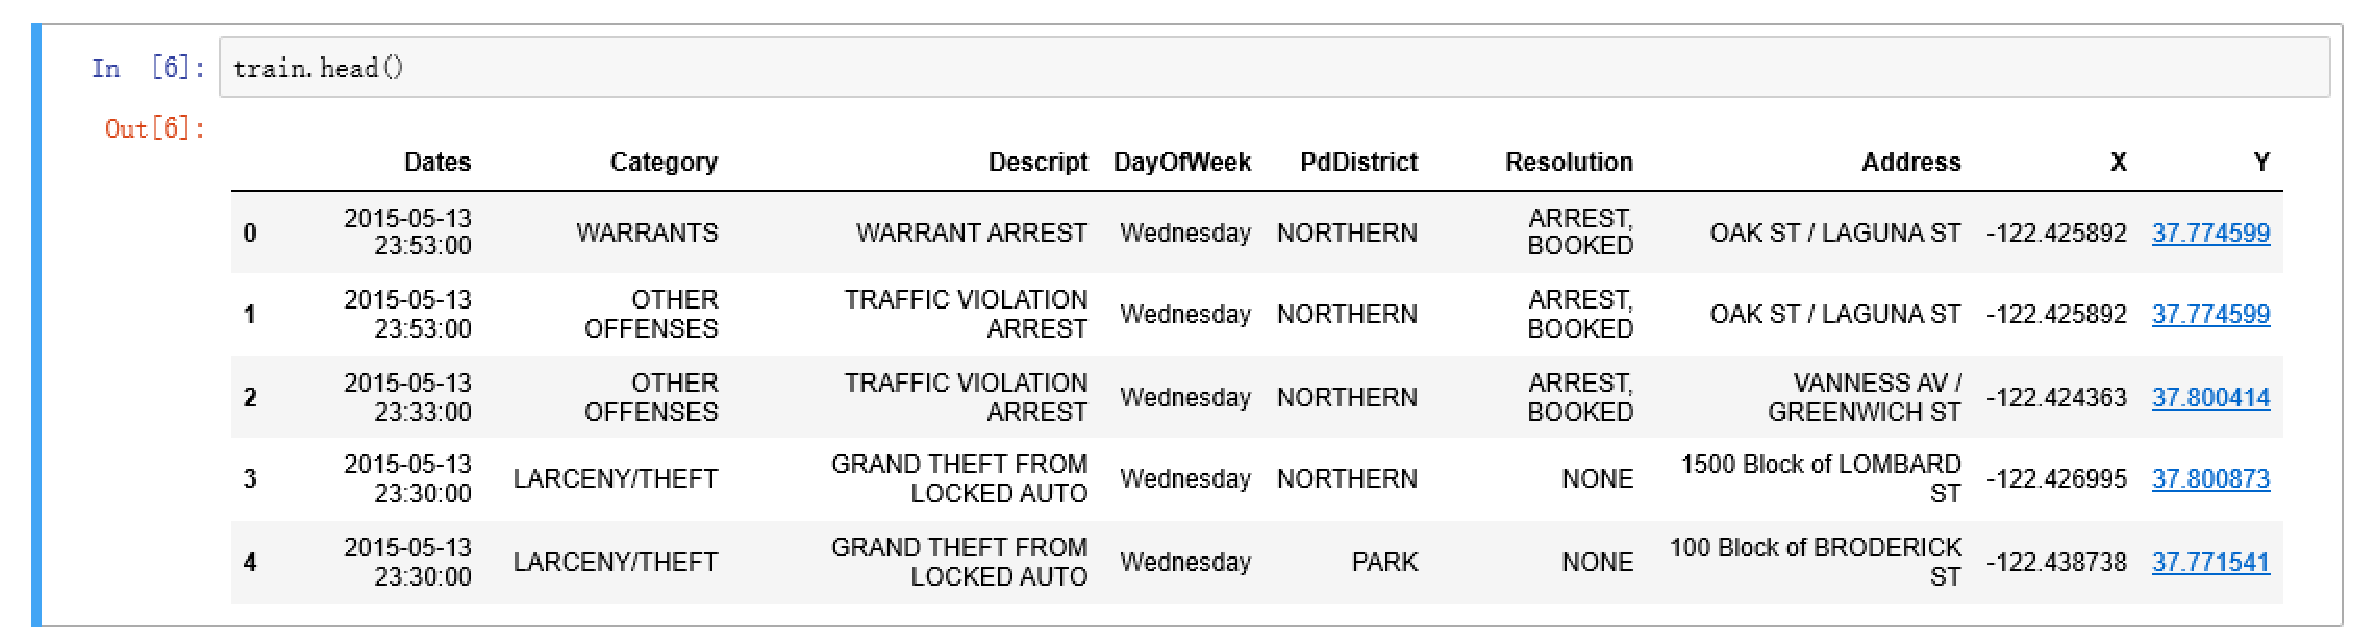
\includegraphics[width=1\textwidth]{kaggle/2.eps}
  \end{figure}
  
  \bigskip
More specifically it includes the following variables.
  \begin{itemize}
    \item Date - timestamp of the crime Incident.
    \item Category - category of the crime incident. (This is our target variable.)
    \item Descript - detailed description of the crime incident
    \item DayOfWeek - the day of the week
    \item PdDistrict - the name of the Police Department District
    \item Resolution - The resolution of the crime incident

  \end{itemize}
\end{slide}
%%
%%==================================================================



\begin{slide}{Features Item}
  \begin{itemize}
    \item Address - the approximate street address of the crime incident
    \item X - Longitude
    \item Y - Latitude
  \end{itemize}
\end{slide}

%%==========================================================================================

\section{Feature Analysis}

%%==========================================================================================
%%

%%
%%===========================================================================================



%%
%%=============================================================================================
\begin{slide}[toc=,bm=]{Feature Analysis}
\begin{itemize}
\item The data set contains nine eigenvalues, the data types are as follows,
 and we can see that the data set contains' object 'variables (also known as strings) 
 that we need to encode.

\end{itemize}

\begin{figure}[htbp]
  \centering
  \begin{minipage}[t]{0.48\textwidth}
    \centering
    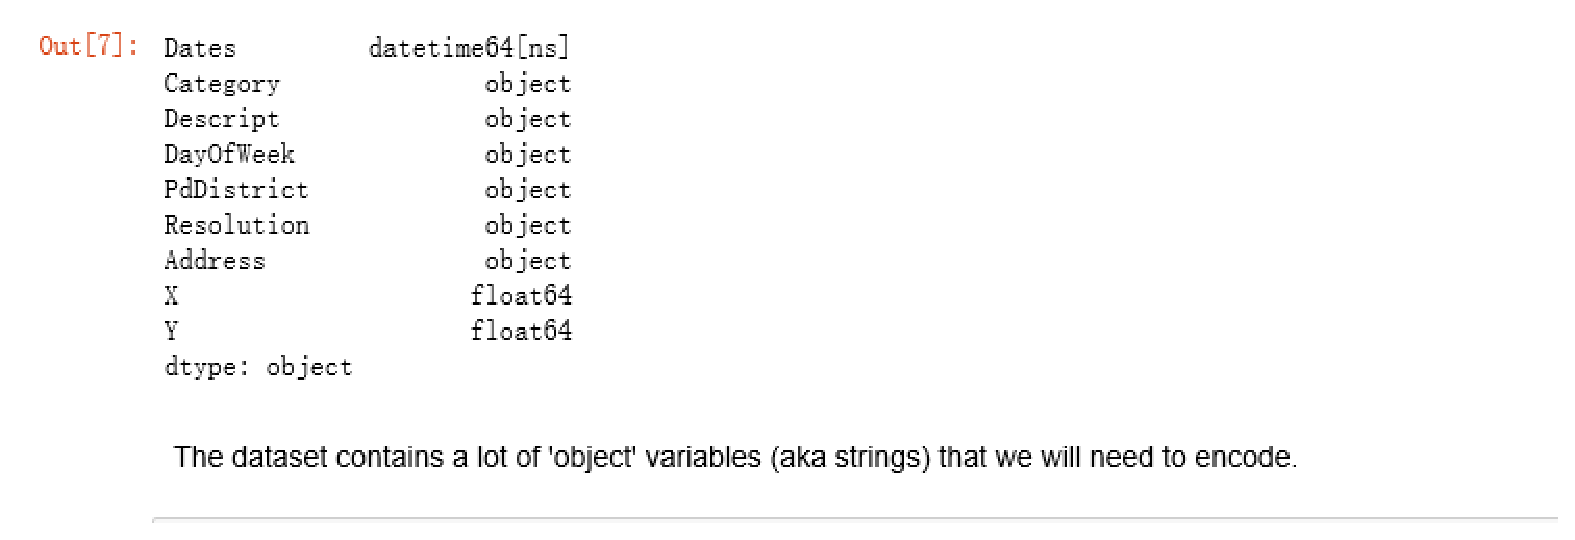
\includegraphics[width=0.8\textwidth]{kaggle/3.eps}
    \vspace{0.4em}
    \caption{ Data Type}
  \end{minipage}
  \begin{minipage}[t]{0.48\textwidth}
    \centering
    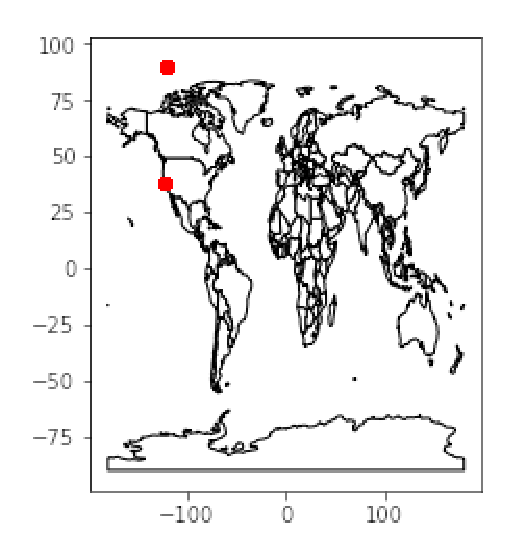
\includegraphics[width=0.6\textwidth]{kaggle/5.eps}
    \vspace{0.4em}
    \caption{}
  \end{minipage}
\end{figure}

The 2,323 copies are duplicates and we need to delete them.
We will also evaluate the position of the data points using the coordinates.
%%==========================================================================================
\begin{note}
In conclusion,
we firstly formalized the problem of
group outlying aspects mining,

Then proposed a novel method GOAM algorithm to address the problem of
group outlying aspects mining,
and the proposed method use pruning to reduce time complexity
while identifying the suitable set of outlying features for the interested group.

Thank you and any question?
\end{note}
%%==========================================================================================

\end{slide}
%%
%%==========================================================================================

\begin{slide}{Feature Analysis}
  There are also some wrong locations in the data set. After analysis, we 
  found a total of 67 wrong messages, which also means that we cannot use
   these 67 wrong messages.
  \begin{figure}
    \centering
    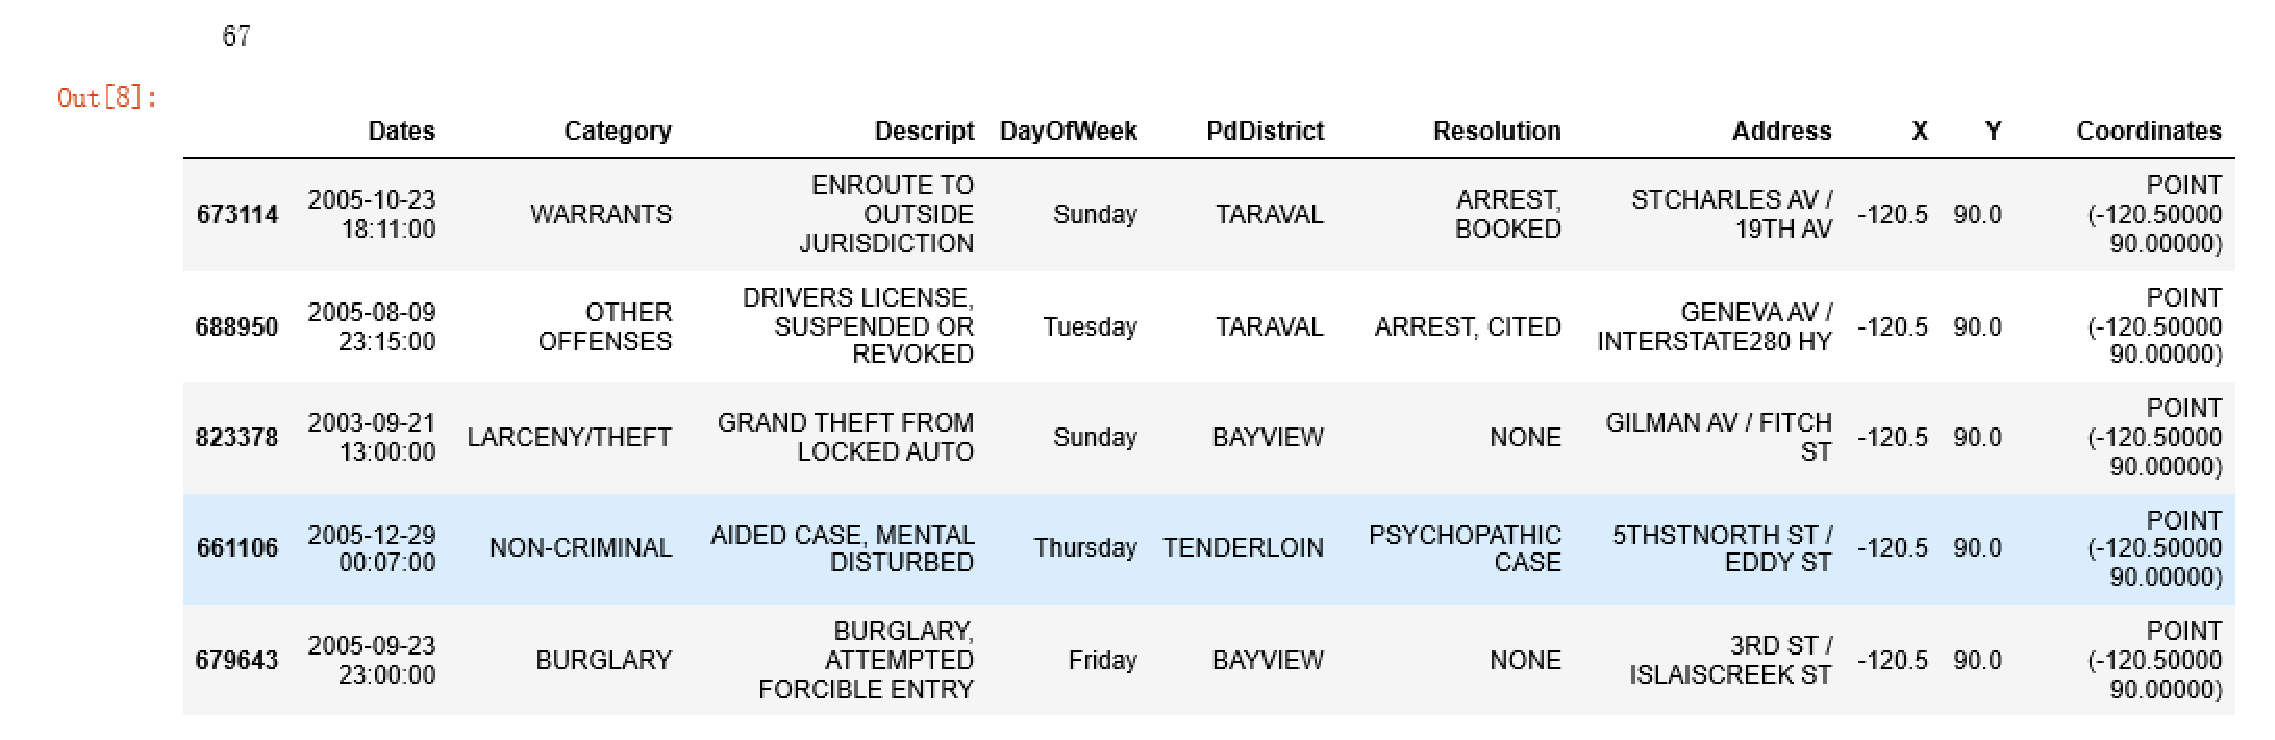
\includegraphics[width=1\textwidth]{kaggle/6.1.eps}
  \end{figure}


\end{slide}
%%
%%===========================================================================================



%%
%%========================================================================

\begin{slide}{Dates \& Day of the week}
  These variables are distributed uniformly between 1/1/2003 to 5/13/2015 (and Monday to Sunday) and split between the training and the testing dataset as mentioned before. We did not notice any anomalies on these variables.
  The median frequency of incidents is 389 per day with a standard deviation of 48.51.
  Also, there is no significant deviation of incidents frequency 
  throughout the week. Thus we do not expect this variable to play a 
  significant role in the prediction.


  \begin{figure}[htbp]
    \centering
    \begin{minipage}[t]{0.48\textwidth}
      \centering
      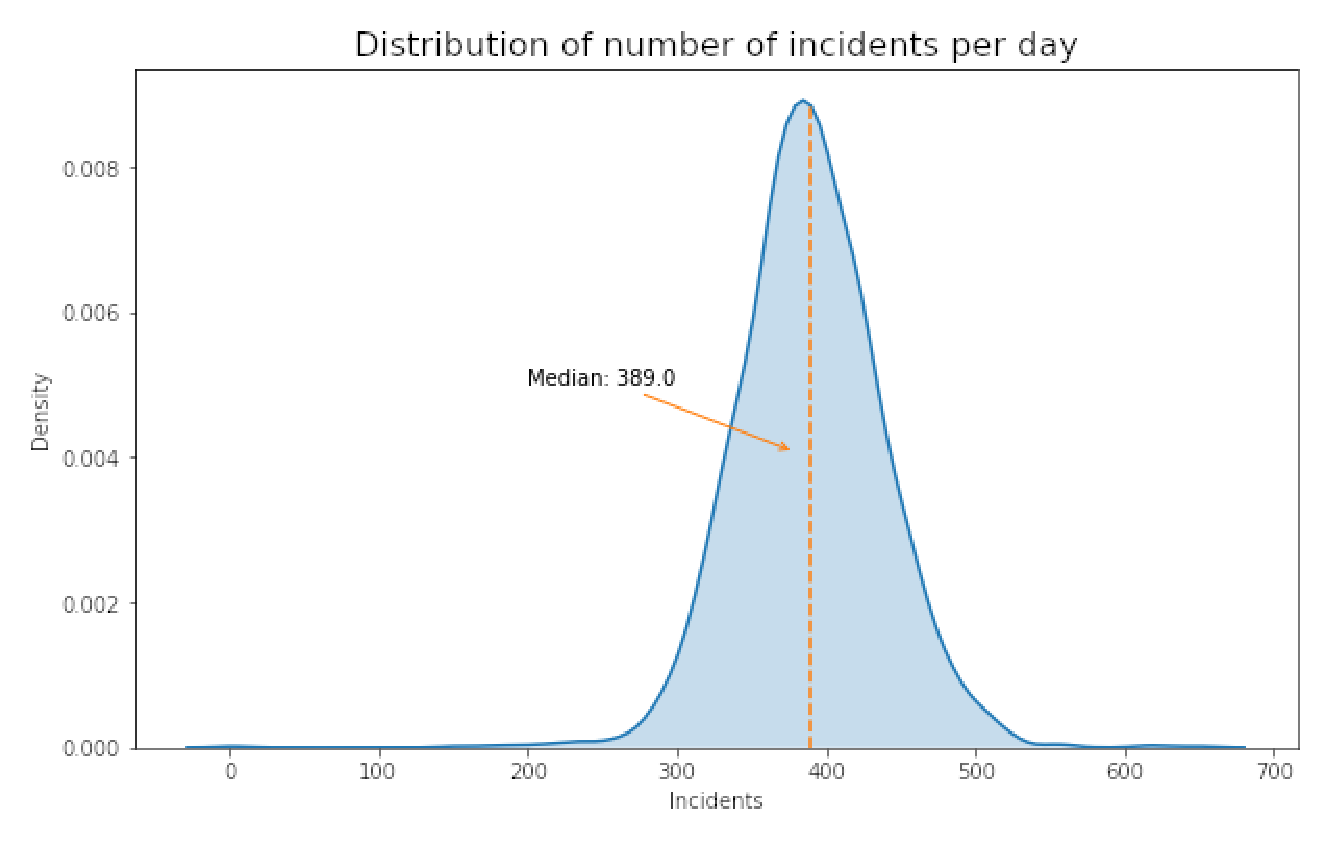
\includegraphics[width=0.8\textwidth]{kaggle/7.1.eps}
      \vspace{0.4em}
      \caption{Dates and Day of the Week}
    \end{minipage}
    \begin{minipage}[t]{0.48\textwidth}
      \centering
      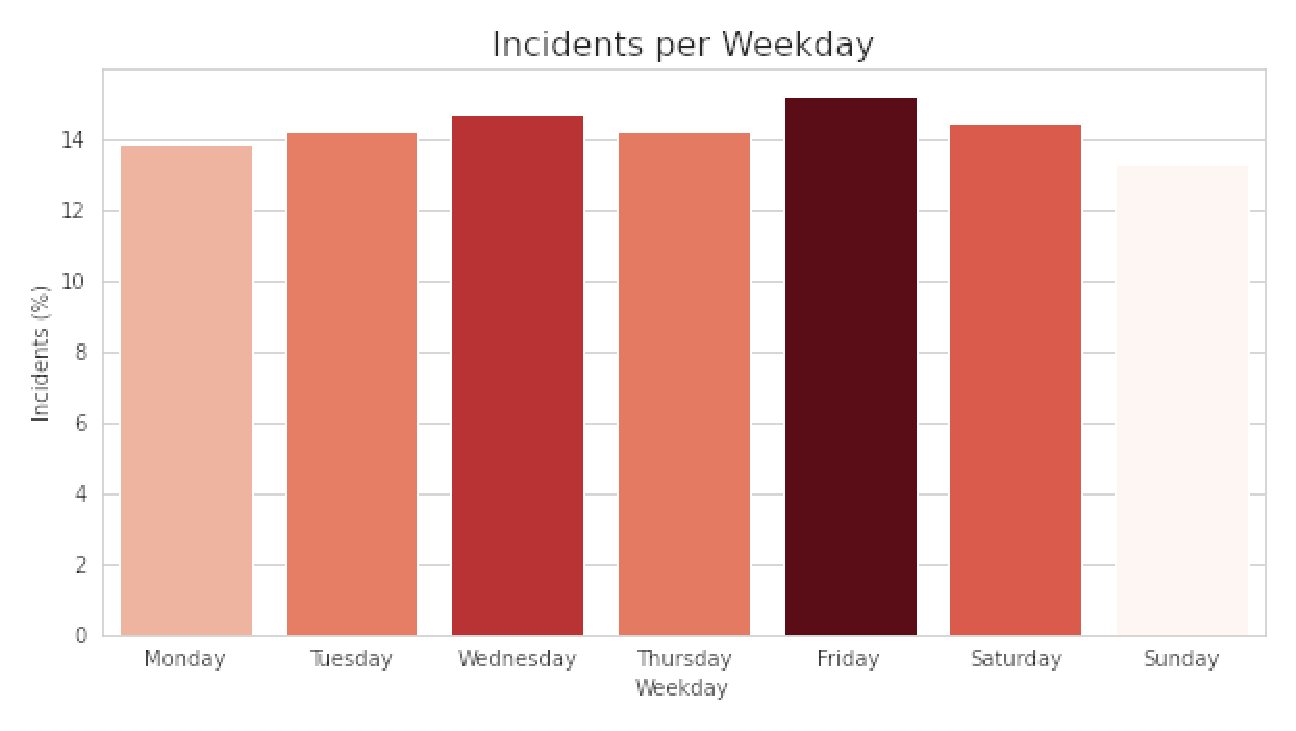
\includegraphics[width=0.8\textwidth]{kaggle/8.1.eps}
      \vspace{0.4em}
      \caption{Per Weekday}
    \end{minipage}
  \end{figure}
\end{slide}

%%
%%%%===============================================================

%%
%%===================================================================



\begin{slide}{Category \& Police District}
  There are 39 discrete categories that the police department file the incidents with the most common being 
  Larceny/Theft (19.91\%), Non/Criminal (10.50\%), and Assault(8.77\%).
  There are significant differences between the different districts of the City with the Southern district 
  having the most incidents (17.87\%) followed by Mission (13.67\%) and Northern (12.00\%).
  \begin{figure}[htbp]
    \centering
    \begin{minipage}[t]{0.48\textwidth}
      \centering
      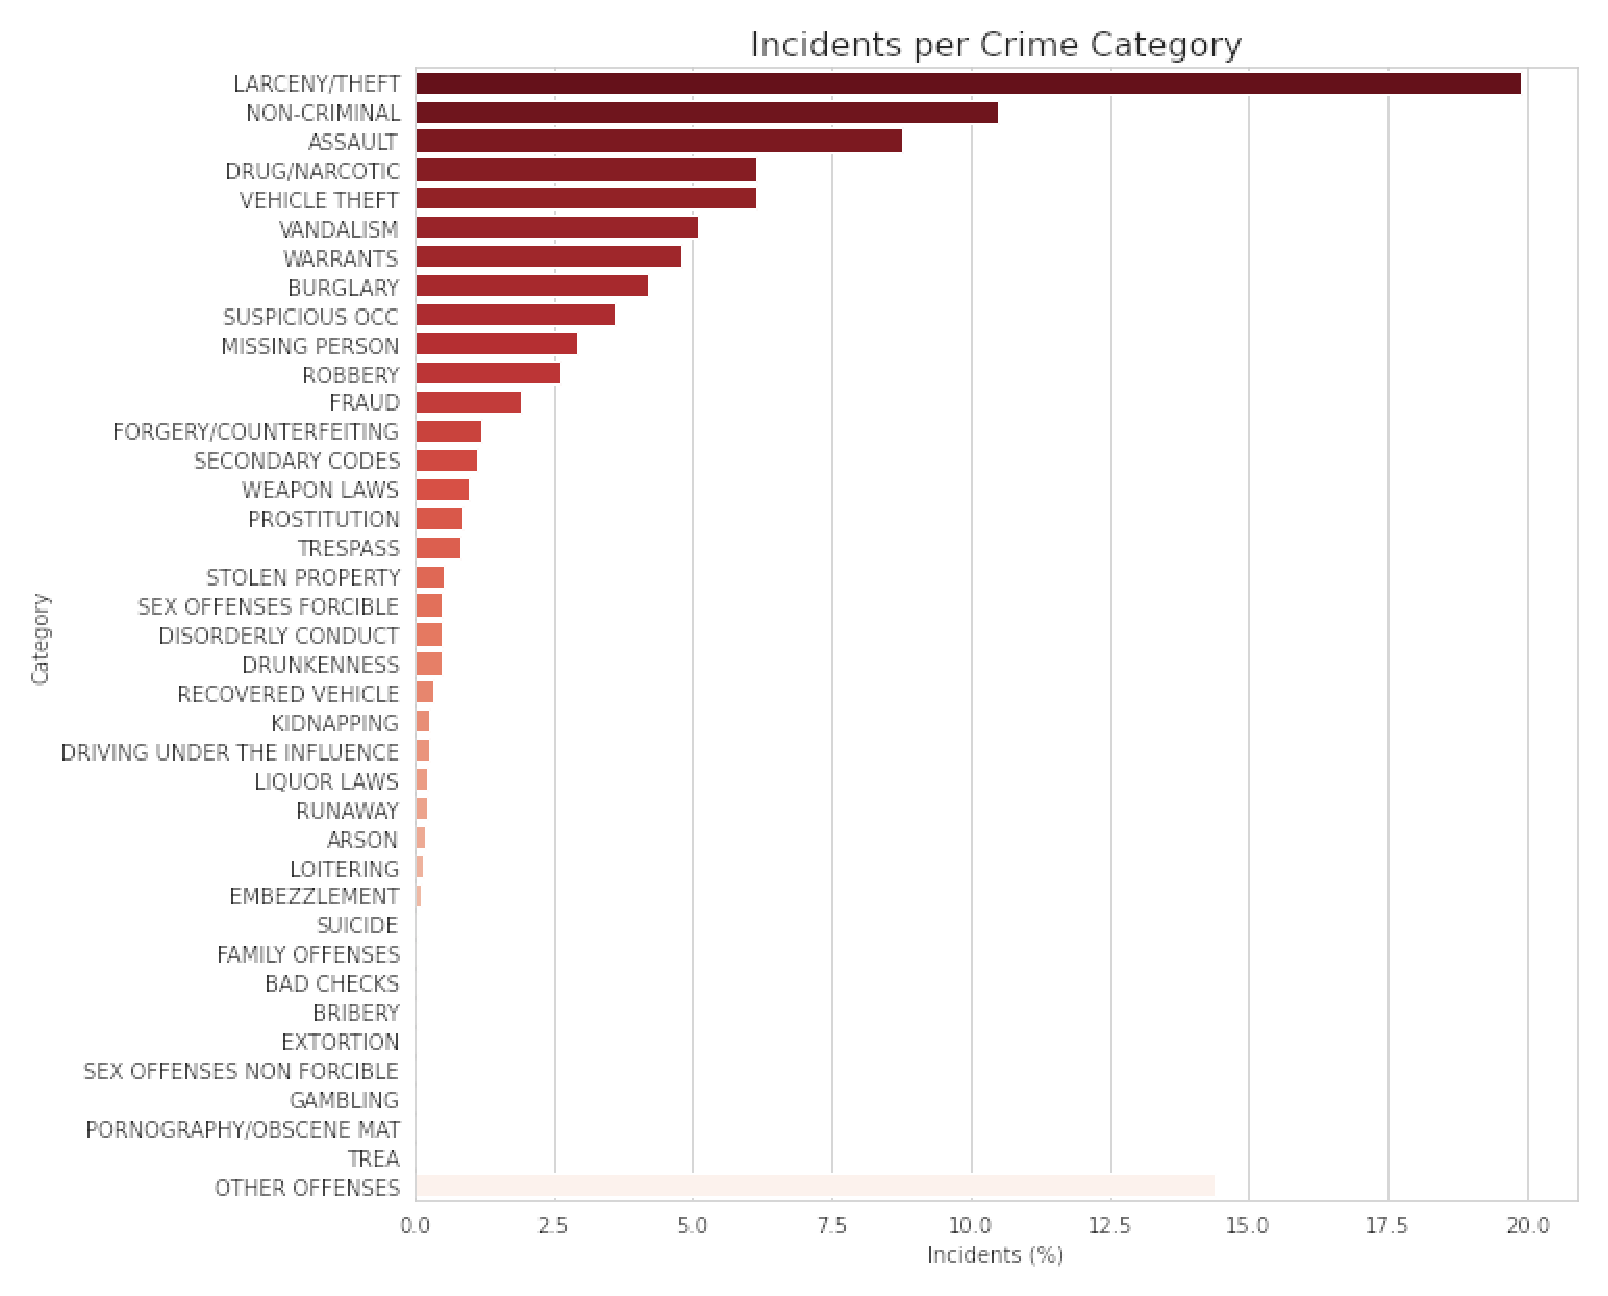
\includegraphics[width=0.7\textwidth]{kaggle/9.eps}
      \vspace{0.4em}
      \caption{Category}
    \end{minipage}
    \begin{minipage}[t]{0.48\textwidth}
      \centering
      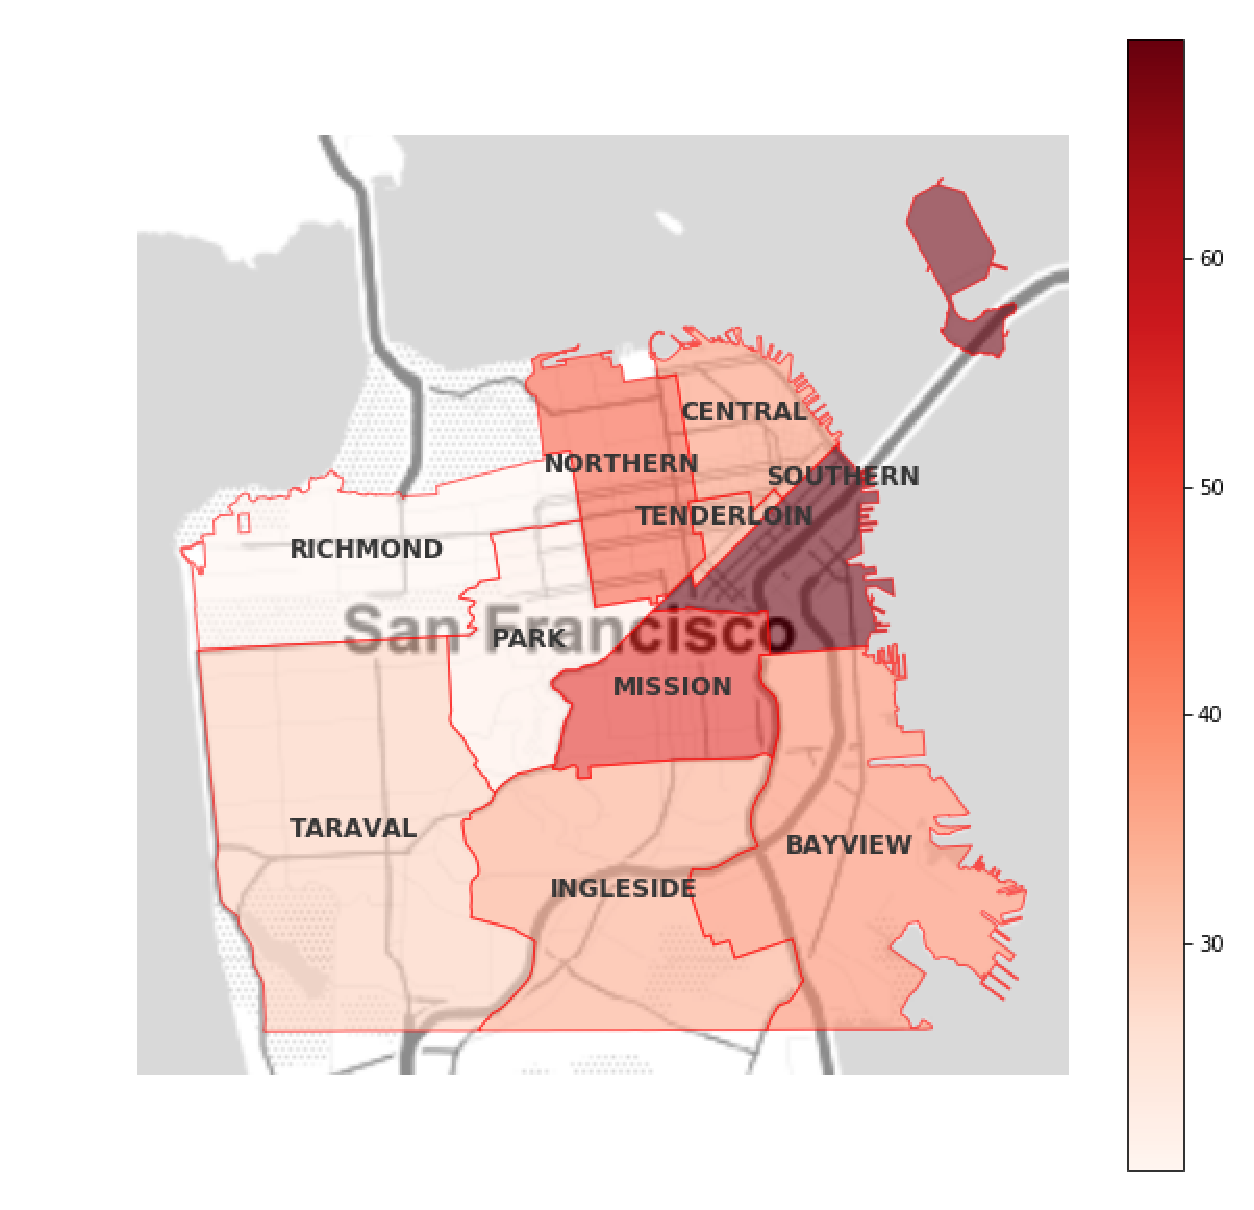
\includegraphics[width=0.7\textwidth]{kaggle/10.eps}
      \vspace{0.4em}
      \caption{Police District}
    \end{minipage}
  \end{figure}
\end{slide}

%%
%%=========================================================================

%%
%%==========================================================================


\begin{slide}{X \& Y}
  \begin{itemize}
  \item Address
Address, as a text field, requires advanced techniques to use 
it for the prediction. Instead in this project, we will use it to 
extract if the incident has happened on the road or in a building block.
\item X - Longitude Y - Latitude
We have tested that the coordinates belong inside the
 boundaries of the city. Although longitude does not contain any
  outliers, latitude includes some 90o values which correspond to the North Pole.
\end{itemize}
\end{slide}

%%
%%==============================================================================

\section{Feature Selection} 

%%===========================================================================================
%%

%%
%%========================================================================================

\begin{slide}{Feature Engineering}
  Then, we created additional features. More specifically:
\begin{itemize}
  \item From the ‘Dates’ field, we extracted the Day, the Month, the
   Year, the Hour, the Minute, the Weekday, and the number of days 
   since the first day in the data.

  \item From the ‘Address’ field we extracted if the incident has taken
   place in a crossroad or on a building block.
\end{itemize}

\begin{figure}
  \centering
  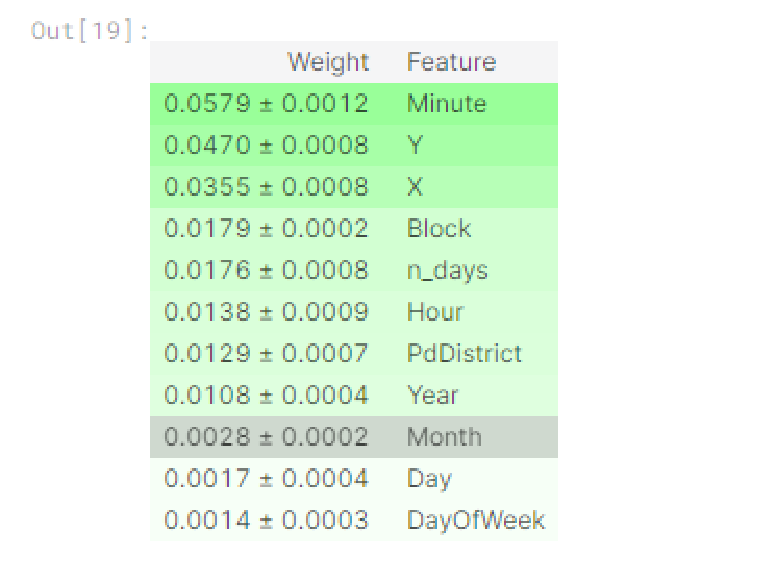
\includegraphics[width=0.5\textwidth]{kaggle/14.eps}
\end{figure}
  
\end{slide}


%%
%%==================================================================================




%%
%%==============================================================================


\section{Modelling}

%%
%%============================================================================================

%%
%%==============================================================================================
\begin{slide}{Calculate the Baseline Value For The Model}
  Since this is a typical multi-classification problem, we 
  can choose to use many kinds of algorithms, including naive
   Bayes, KNN, decision tree and random forest.
\end{slide}

%%
%%===============================================================================================



% TODO: Contact Page

\end{document}

\endinput
